\Gls{ibc} systems operate under different environmental scenarios. In this section, we evaluate the impact of approximation noise on \gls{ibc} performance when operating under these scenarios. Fig.~\ref{fig:env_1} shows the six different environmental scenarios considered for our evaluation. These are commonly encountered driving conditions relevant for \gls{lkas}. 
\begin{figure}[ht]
    \centering
    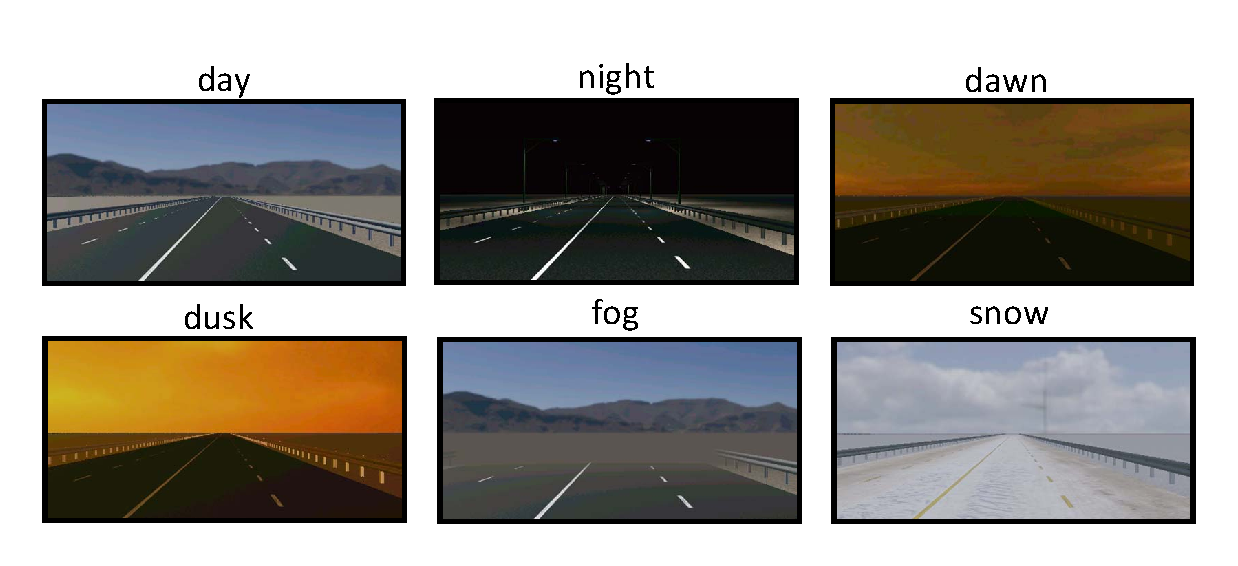
\includegraphics[width= 0.98\textwidth]{figs/scenes_v1.pdf}
    \caption{{Different environmental scenarios considered in this work. The figures are obtained from the \gls{imacs} framework.}}
    \label{fig:env_1}
    \vspace{-2em}
\end{figure}

\begin{figure}[ht]
    \centering
    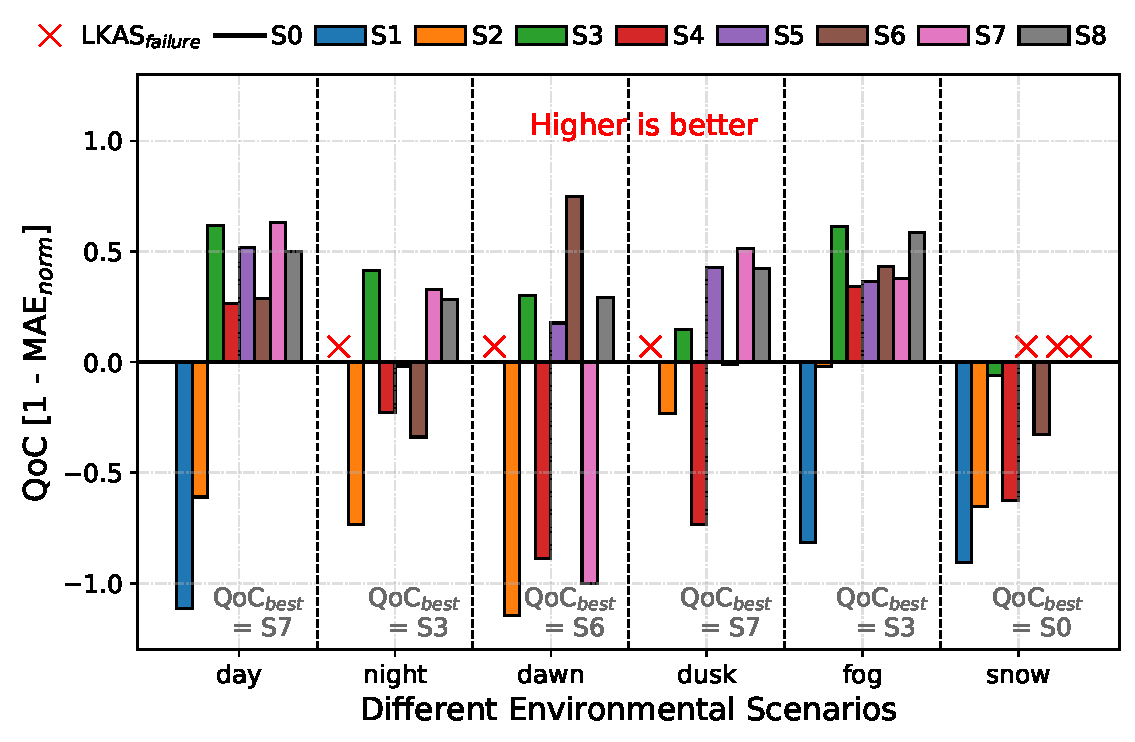
\includegraphics[width= 0.9\textwidth]{figs/robustness2.pdf}
    \caption{{Sensitivity of \gls{qoc} to different approximation settings operating under different environmental scenarios. Results are for Optim 1.}}
    \label{fig:env_2}
    \vspace{-1em}
\end{figure}

\begin{figure}[ht]
    \centering
    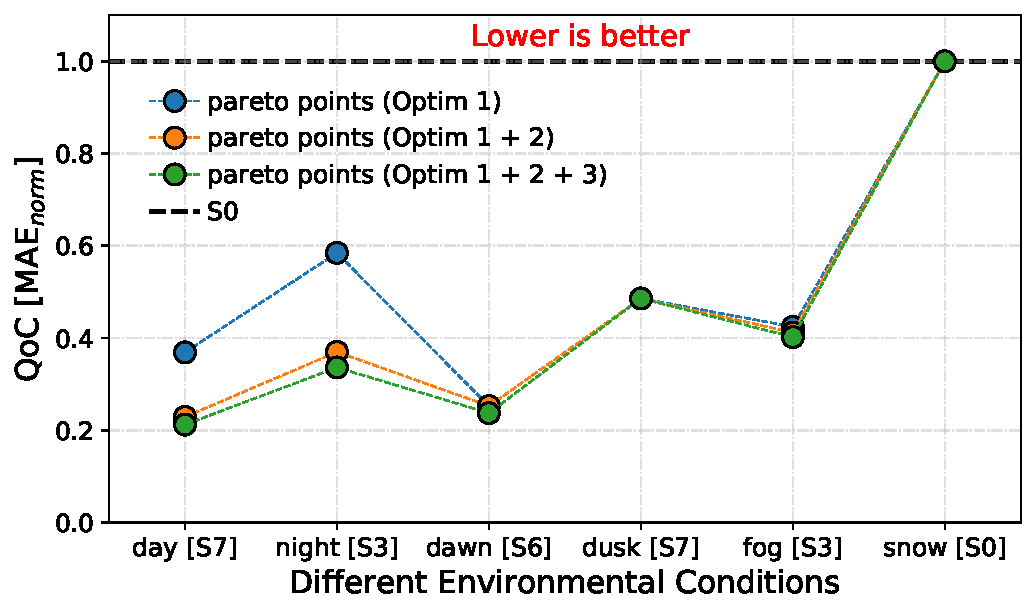
\includegraphics[width= 0.86\textwidth]{figs/lqg2.pdf}
    \captionsetup{width=0.9\linewidth}
    \caption{{\Gls{qoc} improvements due to cross-layer optimizations (Optim 1, 2, 3) across different environmental scenarios.}}
    \label{fig:env_3}
    \vspace{-1em}
\end{figure}

\par Fig.~\ref{fig:env_2} shows the \gls{qoc} sensitivity for \gls{lkas} to approximation settings (S0-S8) when operated under different environmental scenarios. All values are normalized to the S0 \gls{qoc} (baseline). It is observed that the choice of approximation (S1-S8) is critical for better \gls{qoc}. To get the best \gls{qoc}, different approximation settings should be chosen based on the environmental scenario (grey markings in Fig.\ \ref{fig:env_2}). S1 (skipping denoising) fails for night, dawn and dusk, while it performs worse than the baseline for the other scenarios. Similarly, S2 (skipping color map) performs worse than the baseline across all scenarios. This can be explained by the fact thatvthe sampling period for these cases is not improved compared to S0, while the added extra error makes the \gls{qoc} worse. It is also observed that none of the approximation settings (S1-S8) improves over the baseline when operating in a snowy scenario. Settings S5, S7 and S8 lead to \gls{lkas} failure for this case. This is due to the lack of significant difference in pixel intensity between the lane markings and the road region. From this, we can conclude that the impact of approximation error on \gls{lkas} performance is highly sensitive to the operating environment. Dynamic selection of the approximation setting by recognizing the operating environmental scenario is required. 

\par Fig.\ \ref{fig:env_3} shows the impact of the cross-layer optimizations on \gls{qoc} for different scenarios. All the values are normalized to S0 for the corresponding scenario. For this analysis, we choose only the settings that give the best \gls{qoc} per scenario in Fig.\ \ref{fig:env_2}. Firstly, there is no improvement over S0 for snow as none of the approximation settings perform better than the baseline as explained earlier. For all other scenarios, Optim 1 gives \gls{qoc} improvements over S0. For dawn, dusk and fog, we see no/minor incremental \gls{qoc} improvements when we apply Optim 2 and 3 on top of Optim 1. This is because these are challenging cases for proper dynamic thresholding in the \gls{pr} stage. When we add extra noise due to lossy compression, the performance of dynamic thresholding worsens. In case of dawn and fog, the reduced $\tau$ due to Optim 2 and the approximation-aware controller of Optim 3 overpower the impact of worsened \gls{pr} and we get slight \gls{qoc} improvements over Optim 1. However, this is not the case in the dusk. Also, we observe higher \gls{qoc} improvements for the night compared to the day. This is because, for the night, there is a higher difference in intensity between lane pixels and road pixels, compared to that of the day scenario. This results in a better \gls{pr} performance, thus, larger \gls{qoc} improvements.

We considered six different environmental scenarios most relevant to \gls{lkas}. It is worth noting that our approach is applicable to a combination of these scenarios as well. For instance, a segment of road with multiple tunnels can be handled by dynamically switching from a day to a night scenario and vice versa. Dynamic adaptation to environmental scenarios fits seamlessly in the \gls{spade} design philosophy that is already scenario-driven.